\documentclass{article}
\usepackage{amsmath}
\usepackage{amssymb}
\usepackage{graphicx}
\usepackage{color}
\usepackage{enumitem}
\usepackage[margin=0.5in]{geometry}
\usepackage{karnaugh-map}


\title{MATH 318, Assignment 3}
\author{Kyle Rubenok, 260667187}
\date{October 2019}

\begin{document}

\maketitle

    \begin{enumerate}
        \item 
            \begin{enumerate}
                \item
                    \begin{tabular}{ c  c | c  c  c  c  c  c }
                    p & q & ( & $\neg$ & p & $\rightarrow$ & q & )\\
                    \hline 
                    $\top$ & $\top$ &  & $\perp$ & $\top$ & \textcolor{red}{$\top$} & $\top$ & \\
                    $\top$ & $\perp$ &  & $\perp$ & $\top$ & \textcolor{red}{$\top$} & $\perp$ & \\
                    $\perp$ & $\top$ &  & $\top$ & $\perp$ & \textcolor{red}{$\top$} & $\top$ & \\
                    $\perp$ & $\perp$ &  & $\top$ & $\perp$ & \textcolor{red}{$\perp$} & $\perp$ & \\
                    \end{tabular}
                \item
                    \begin{tabular}{@{ }c@{ }@{ }c | c@{ }@{}c@{}@{ }c@{ }@{ }c@{ }@{ }c@{ }@{}c@{}@{ }c@{ }    @{ }c@{ }@{ }c@{ }@{ }c} p & q &  & ( & p & $\land$ & q & ) & $\lor$ & $\neg$ & p & \\
                    \hline 
                    $\top$ & $\top$ &  &  & $\top$ & $\top$ & $\top$ &  & \textcolor{red}{$\top$} & $\bot$ &     $\top$ & \\
                    $\top$ & $\bot$ &  &  & $\top$ & $\bot$ & $\bot$ &  & \textcolor{red}{$\bot$} & $\bot$ &     $\top$ & \\
                    $\bot$ & $\top$ &  &  & $\bot$ & $\bot$ & $\top$ &  & \textcolor{red}{$\top$} & $\top$ &     $\bot$ & \\
                    $\bot$ & $\bot$ &  &  & $\bot$ & $\bot$ & $\bot$ &  & \textcolor{red}{$\top$} & $\top$ &     $\bot$ & \\
                    \end{tabular}
                \item
                    \begin{tabular}{@{ }c@{ }@{ }c | c@{ }@{ }c@{ }@{ }c@{ }@{}c@{}@{ }c@{ }@{ }c@{ }@{ }c@ { }@{ }c@{ }@{}c@{}@{ }c}
                    p & q &  & p & $\rightarrow$ & ( & $\neg$ & p & $\rightarrow$ & q & ) & \\
                    \hline 
                    $\top$ & $\top$ &  & $\top$ & \textcolor{red}{$\top$} &  & $\bot$ & $\top$ & $\top$ &   $\top$ &  & \\
                    $\top$ & $\bot$ &  & $\top$ & \textcolor{red}{$\top$} &  & $\bot$ & $\top$ & $\top$ &   $\bot$ &  & \\
                    $\bot$ & $\top$ &  & $\bot$ & \textcolor{red}{$\top$} &  & $\top$ & $\bot$ & $\top$ &   $\top$ &  & \\
                    $\bot$ & $\bot$ &  & $\bot$ & \textcolor{red}{$\top$} &  & $\top$ & $\bot$ & $\bot$ &   $\bot$ &  & \\
                    \end{tabular}
                \item
                    \begin{tabular}{@{ }c@{ }@{ }c | c@{ }@{ }c@{ }@{ }c@{ }@{}c@{}@{ }c@{ }@{ }c@{ }@{}c@{}    @{ }c@{ }@{ }c@{ }@{}c@{}@{ }c@{ }@{ }c@{ }@{ }c@{ }@{}c@{}@{}c@{}@{}c@{}@{ }c}
                    p & q &  & q & $\lor$ & ( & p & $\rightarrow$ & ( & q & $\land$ & ( & p & $\rightarrow$ &  q & ) & ) & ) & \\
                    \hline 
                    $\top$ & $\top$ &  & $\top$ & \textcolor{red}{$\top$} &  & $\top$ & $\top$ &  & $\top$ &     $\top$ &  & $\top$ & $\top$ & $\top$ &  &  &  & \\
                    $\top$ & $\bot$ &  & $\bot$ & \textcolor{red}{$\bot$} &  & $\top$ & $\bot$ &  & $\bot$ &     $\bot$ &  & $\top$ & $\bot$ & $\bot$ &  &  &  & \\
                    $\bot$ & $\top$ &  & $\top$ & \textcolor{red}{$\top$} &  & $\bot$ & $\top$ &  & $\top$ &     $\top$ &  & $\bot$ & $\top$ & $\top$ &  &  &  & \\
                    $\bot$ & $\bot$ &  & $\bot$ & \textcolor{red}{$\top$} &  & $\bot$ & $\top$ &  & $\bot$ &     $\bot$ &  & $\bot$ & $\top$ & $\bot$ &  &  &  & \\
                    \end{tabular}
            \end{enumerate}
            C is the only tautology. 
        \item 
            \begin{enumerate}
                \item 
                    $\neg p \lor q$ 
                    \newline 
                    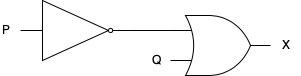
\includegraphics{./2a.png}
                \item 
                    $p \lor q$ 
                    \newline 
                    
\includegraphics{./2b.png}
            \end{enumerate}
        \item
            \begin{enumerate}
                \item DNF
                $$p \lor r$$
                \item CNF
                $$p \lor r$$
            \end{enumerate}
        \item
            \begin{enumerate}[label=\arabic*)]
                \item $p \rightarrow q$ with only NAND
                \newline
                \begin{tabular}{@{ }c@{ }@{ }c | c@{ }@{}c@{}@{}c@{}@{ }c@{ }@{ }c@{ }@{ }c@{ }@{}c@{}@{ }c@{ }@{ }c@{ }@{}c@{}@{ }c@{ }@{}c@{}@{ }c@{ }@{ }c@{ }@{ }c@{ }@{}c@{}@{ }c}
                    p & q &  & ( & ( & p & $NAND$ & q & ) & $NAND$ & p & ) & $\leftrightarrow$ & ( & p & $\rightarrow$ & q & ) & \\
                    \hline 
                    T & T &  &  &  & T & F & T &  & T & T &  & \textcolor{red}{T} &  & T & T & T &  & \\
                    T & F &  &  &  & T & T & F &  & F & T &  & \textcolor{red}{T} &  & T & F & F &  & \\
                    F & T &  &  &  & F & T & T &  & T & F &  & \textcolor{red}{T} &  & F & T & T &  & \\
                    F & F &  &  &  & F & T & F &  & T & F &  & \textcolor{red}{T} &  & F & T & F &  & \\
                    \end{tabular}
                \item $(p \land q)\lor \neg p$ with only NOR
                \newline
                \begin{tabular}{@{ }c@{ }@{ }c | c@{ }@{}c@{}@{}c@{}@{}c@{}@{ }c@{ }@{ }c@{ }@{ }c@{ }@{}c@{}@{ }c@{ }@{ }c@{ }@{}c@{}@{ }c@{ }@{}c@{}@{}c@{}@{ }c@{ }@{ }c@{ }@{ }c@{ }@{}c@{}@{ }c@{ }@{ }c@{ }@{}c@{}@{}c@{}@{ }c@{ }@{}c@{}@{}c@{}@{ }c@{ }@{ }c@{ }@{ }c@{ }@{}c@{}@{ }c@{ }@{ }c@{ }@{ }c@{ }@{}c@{}@{ }c}
                    p & q &  & ( & ( & ( & p & $NOR$ & p & ) & $NOR$ & q & ) & $NOR$ & ( & ( & p & $NOR$ & p & ) & $NOR$ & q & ) & ) & $\leftrightarrow$ & ( & ( & p & $\land$ & q & ) & $\lor$ & $\neg$ & p & ) & \\
                    \hline 
                    T & T &  &  &  &  & T & F & T &  & F & T &  & T &  &  & T & F & T &  & F & T &  &  & \textcolor{red}{T} &  &  & T & T & T &  & T & F & T &  & \\
                    T & F &  &  &  &  & T & F & T &  & T & F &  & F &  &  & T & F & T &  & T & F &  &  & \textcolor{red}{T} &  &  & T & F & F &  & F & F & T &  & \\
                    F & T &  &  &  &  & F & T & F &  & F & T &  & T &  &  & F & T & F &  & F & T &  &  & \textcolor{red}{T} &  &  & F & F & T &  & T & T & F &  & \\
                    F & F &  &  &  &  & F & T & F &  & F & F &  & T &  &  & F & T & F &  & F & F &  &  & \textcolor{red}{T} &  &  & F & F & F &  & T & T & F &  & \\
                    \end{tabular}
            \end{enumerate}
        \item The formula is even when $n \geq 2$ and n is an even number. We will proove this by induction on n. 
        \newline
        % \item BOLD THE HEADERS> 
        \textbf{Base Case:} take n = 2. This follows from the truth table. 
        \newline
        \begin{tabular}{@{ }c | c@{ }@{ }c@{ }@{ }c@{ }@{ }c@{ }@{ }c}
            p &  & p & $\rightarrow$ & p & \\
            \hline 
            T &  & T & \textcolor{red}{T} & T & \\
            F &  & F & \textcolor{red}{T} & F & \\
            \end{tabular}
        \newline
        \textbf{Induction Step:} Taking that this holds for any other $n$, we will show that it holds for $n+2$. Since we can assume that any formula with an even $n$ number of $p$'s, we need to show that $(T \rightarrow p) \rightarrow p$ is also true. This clearly follows from the truth table.
        \item \textbf{$\leftarrow$} Assuming that every variable in $\varphi$ occurs $n$ times, where $n$ is an even number. Once again, take that each $\varphi_i$ also appear exactly $m$ times, where $m$ is also an even number. All instances of $\varphi_i$ may be grouped in pairs connected by a $\leftrightarrow$ in the following manner:
        $$(\varphi_1 \leftrightarrow \varphi_1 )\leftrightarrow (\varphi_2 \leftrightarrow \varphi_2 )\leftrightarrow [....](\varphi_n \leftrightarrow \varphi_n )$$
        This would require that any individual $(\varphi_i \leftrightarrow \varphi_i )$ is a tautology making the entire construction a tautology as well. 
        \textbf{$\rightarrow$} Let $\varphi$ be a tautology. 
        \newline
        We can write a formula of the binconditional equivalence of $\varphi_i$ where $0\leq i\leq n$ and each $\varphi_i$ is a variable or a negation or a variable. If we assume that at least one of the $\varphi_i$ appears an odd number of times, let's assume it's $\varphi_j$. Taking the same formula contruction as above but appending the following:
        $$(\varphi_1 \leftrightarrow \varphi_1 )\leftrightarrow (\varphi_2 \leftrightarrow \varphi_2 )\leftrightarrow [....](\varphi_n \leftrightarrow \varphi_n )\leftrightarrow \varphi_j $$
        The created a contradiction as the formula is no longer a tautology requiring that should $\varphi$ be a tautology, it must contain an even number of $\varphi_i$.
        \item
            Drawing the karnaugh map as follows:
            \newline
            \begin{karnaugh-map}[4][4][1][$rs$][$pq$]
                \maxterms{6,7,15,14}
                \minterms{0,1,2,3,4,5,8,9,10,11,12,13}
                \implicant{0}{2}
                \implicant{0}{9}
                \implicant{8}{10}
            \end{karnaugh-map}
            \newline
            Giving the following: $f = \neg r \lor (\neg p \land \neg q)\lor (p\land \neg q)$
        \item The set $\{\lor , \land \}$ is not functionally complete. We can prove this by showing it is not 1-complete. Take the $\neg$ operator. Regardless of what input we give to any combination of $\{\lor , \land \}$, ${T \land T \leftrightarrow T}$ and ${F \land F \leftrightarrow F}$. There is no way to invert the input and achieve equivalence to $\neg$
        \item Take for example the formula $p \lor \neg p$. If we attempt to replicate this with the set $\{\oplus\}$. Considering the operations available, it's clear that outside of the identity function of $p = T$ any formulas constructed with combinations of $p$ and $\oplus$ such as $p \oplus p$ and so on will be logically false. This makes replicating the formula $p \lor \neg p$ and many others impossible. Thus $\{\oplus\}$ is not functionally complete. 
    \end{enumerate}
\end{document}